\documentclass[12pt]{article}

%%% --- PACKAGES --- %%%
\usepackage{amsmath}
\usepackage{amssymb}
\usepackage{amsthm}
\usepackage{float}
\usepackage{tikz,graphicx,pgfplots}
\usetikzlibrary{patterns,decorations.pathmorphing,positioning}
\pgfplotsset{compat=1.10}
\usepgfplotslibrary{fillbetween}
\usepackage{xcolor}
\usepackage{verbatim}
\usepackage{listings}
\usepackage{enumitem}
\usepackage{booktabs}

%%% --- PAGE LAYOUT --- %%%
\setlength{\textwidth}{168.0truemm}
\setlength{\textheight}{255.0truemm}
\setlength{\oddsidemargin}{-4.0mm}
\setlength{\evensidemargin}{-4.0mm}
\setlength{\topmargin}{-22.0truemm}
\parindent=0mm
\parskip=2mm
\pagestyle{empty}

%%% --- MATH OPERATORS --- %%%
\DeclareMathOperator\artanh{artanh}
\DeclareMathOperator\arsinh{arsinh}
\DeclareMathOperator\arcosh{arcosh}
\DeclareMathOperator\sech{sech}
\newcommand{\ds}{\displaystyle}

\newenvironment{solution}{%
    \par\vspace{4pt}%
    \noindent\rule{\linewidth}{0.3pt}%
    \par\smallskip%
    \noindent\textit{Solution.}\par\smallskip%
}{%
    \par\noindent\rule{\linewidth}{0.3pt}%
    \par\vspace{6pt}%
}

% Placeholder vertical space 
\newcommand{\answerspace}[1][6cm]{\vspace{#1}}

%%% -------------------------------------------------------- %%%
\begin{document}

%%% --- HEADER --- %%%
\begin{center}
    {\bf COLLEGE OF SCIENCE}
\end{center}
\centerline{\large\bf PHYS2020}     
\vspace{0.1cm}
\centerline{\large\bf Simulation Plan} 
\vspace{0.1cm}
\centerline{\large\bf Semester One 2026}
\vspace{3mm}
\hrule
\vspace{3mm}

\begin{tabular}{rl}
    & Family name: Lukacs \\[6pt]
    & Given names: Matthew David Carmel\\[6pt]
    & Student number: u8507410\\[6pt]
\end{tabular}

\vspace{4mm}
\hrule
\vspace{4mm}



\section{Project Plan: Simulation of Brownian Motion}

\subsection{Overview}
This project aims to simulate Brownian motion using a computational random walk model and to demonstrate how diffusion emerges from microscopic randomness. The simulation will track the motion of particles in two dimensions and compare numerical results with theoretical predictions, particularly the linear relationship between mean squared displacement (MSD) and time.\\

This was particularly inspired by my labwork in PHYS2013.

\subsection{Goals}
The goals of this project are:
\begin{itemize}
    \item To implement a randomised 2D walk simulation for multiple particles
    \item to calculate and analyse MSD as f(t)
    \item verify proportionality between MSD and t
    \item to investigate the effects of varying parameters like step-size. step-size is related to temperature too, as the further the particles move during the step-size, the faster they must be going, so they have a higher kinetic energy, which is proportional to temp.
\end{itemize}

\subsection{Methodology}
The simulation will model $N$ particles undergoing discrete-time random motion in a 2D domain. We will calculate $\delta x$ and $\delta y$ as well as $\delta r$ using timesteps.
The mean squared displacement will be calculated.
A linear fit will be applied to MSD vs time data to extract the diffusion coefficient $D$, based on:
\[
\text{MSD}(t) = 4Dt
\]

These equations come from Einstein, and the assumption is we can treat x and y as independent due to orthogonality and pool them.

\subsection{Implementation}
The simulation will be implemented in Python. The program will:
\begin{enumerate}
    \item Initialise particle positions at the origin.
    \item Iterate over time steps, updating positions randomly.
    \item Store particle trajectories.
    \item Compute and plot MSD as a function of time.
\end{enumerate}

\subsection{Extensions}
To enhance the project, several extensions may be implemented:
\begin{itemize}
    \item Varying step size to simulate temperature dependence.
    \item Introducing boundaries or obstacles.
    \item Adding a constant drift velocity to simulate external forces.
\end{itemize}

\subsection{Expected Outcomes}
The simulation is expected to demonstrate a linear relationship between MSD and time, validating the diffusion model. Deviations from ideal behaviour will be analysed and discussed in terms of numerical limitations and finite sampling effects. I will compare the python results to theoretical results.

\subsection{Diagram of Simulation Process}

\begin{center}
\begin{tikzpicture}[node distance=2.5cm, every node/.style={draw, rectangle, rounded corners}]
\node (start) {Initialise Particles};
\node (update) [below of=start] {Update Positions Randomly};
\node (store) [below of=update] {Store Positions};
\node (msd) [below of=store] {Compute MSD};
\node (loop) [below of=msd] {Next Time Step};

\draw[->] (start) -- (update);
\draw[->] (update) -- (store);
\draw[->] (store) -- (msd);
\draw[->] (msd) -- (loop);
\draw[->] (loop) -- ++(3,0) -- ++(0,8) -- (update);
\end{tikzpicture}
\end{center}

\subsection{What I've done so far}
I have now set up a github repository which is also linked to my google drive\\
https://github.com/carmel3141/Brownian-Motion-Simulation-PHYS2020\\
I have tested a few commits to see if i remember how to use github.
I know what formulas I will be testing from the Brownian Motion Lab manual, and i will be using numpy and matplot in python to implement it. The rng generator in python should suffice, and it should be quite quick to set something very basic up, then I will scale it up from there. I know I will need to compare these results to real results, and I might be able to reference my brownian motion laboratory results even, perhaps. 

\subsection{Challenges and Limitations}

challenges may arise in developent. it might be difficult to ensure that the random walk accurately represents physical diffusion. im planning on making the model based off those aforementioned x and y values which according to einstein will form a normal, gaussian distribution, so consequently the x and y values will depend on sigma squared, which will also consequently still be a proxy with temperature, so we will need an accurate sigma.\\

this approach is a simplification of real Brownian motion. The simulation does not explicitly include forces, particle collisions, or interactions with a surrounding medium, the time step will also effect accuracy.

Another challenge lies in statistical accuracy. Since the mean squared displacement is an average over many particles, a sufficiently large number of particles and time steps is required to obtain smooth, reliable results. Finite sampling can lead to fluctuations that obscure the expected linear relationship between MSD and time.

Finally, the quality of the random number generator may affect the simulation. Poor randomness could introduce unintended correlations in particle motion. These limitations will be considered when analysing results, and any deviations from theoretical predictions will be discussed in terms of these factors.
\subsection{Conclusion}
This project provides a computational framework for exploring diffusion. By combining simulation with theoretical analysis, it demonstrates how simple random motion leads to predictable macroscopic behaviour.
\end{document}